%----------------------------------------------------------------------------------------------------------------
% Codificação: UTF-8
% LaTeX:  abnTeX2          
% ---------------------------------------------------------------------------------------------------------------


% CARREGA CLASSE PERSONALIZADA DA UTFPR--------------------------------------------------------------------------
\documentclass[%twoside,                   % Impressão em frente e verso
    	        oneside,                   % Impressão apenas frente
]{configuracoes/utfpr-abntex2}


% INCLUI ARQUIVOS DE CONFIGURAÇÕES-------------------------------------------------------------------------------
% REFERÊNCIAS------------------------------------------------------------------
\usepackage[%
    alf,
    abnt-emphasize=bf,
    bibjustif,
    recuo=0cm,
    abnt-url-package=url,       % Utiliza o pacote url
    abnt-refinfo=yes,           % Utiliza o estilo bibliográfico abnt-refinfo
    abnt-etal-cite=3,
    abnt-etal-list=3,
    abnt-thesis-year=final
]{abntex2cite}                  % Configura as citações bibliográficas conforme a norma ABNT

% PACOTES----------------------------------------------------------------------
\usepackage[utf8]{inputenc}                                 % Codificação do documento
\usepackage[T1]{fontenc}                                    % Seleção de código de fonte
\usepackage{booktabs}                                       % Réguas horizontais em tabelas
\usepackage{color, colortbl}                                % Controle das cores
\usepackage{float}                                          % Necessário para tabelas/figuras em ambiente multi-colunas
\usepackage{graphicx}                                       % Inclusão de gráficos e figuras
\usepackage{icomma}                                         % Uso de vírgulas em expressões matemáticas
\usepackage{indentfirst}                                    % Indenta o primeiro parágrafo de cada seção
\usepackage{microtype}                                      % Melhora a justificação do documento
\usepackage{multirow, array}                                % Permite tabelas com múltiplas linhas e colunas
\usepackage{subeqnarray}                                    % Permite subnumeração de equações
\usepackage{lastpage}                                       % Para encontrar última página do documento
\usepackage{verbatim}                                       % Permite apresentar texto tal como escrito no documento, ainda que sejam comandos Latex
\usepackage{amsfonts, amssymb, amsmath}                     % Fontes e símbolos matemáticos
\usepackage[algoruled, portuguese]{algorithm2e}             % Permite escrever algoritmos em português
%\usepackage[scaled]{helvet}                                % Usa a fonte Helvetica
\usepackage{times}                                          % Usa a fonte Times
%\usepackage{palatino}                                      % Usa a fonte Palatino
%\usepackage{lmodern}                                       % Usa a fonte Latin Modern
\usepackage[bottom]{footmisc}                               % Mantém as notas de rodapé sempre na mesma posição
\usepackage{ae, aecompl}                                    % Fontes de alta qualidade
\usepackage{latexsym}                                       % Símbolos matemáticos
\usepackage{lscape}                                         % Permite páginas em modo "paisagem"
%\usepackage{picinpar}                                      % Dispor imagens em parágrafos
%\usepackage{scalefnt}                                      % Permite redimensionar tamanho da fonte
%\usepackage{subfig}                                        % Posicionamento de figuras
%\usepackage{upgreek}                                       % Fonte letras gregas

% Redefine a fonte para uma fonte similar a Arial (fonte Helvetica)
\renewcommand*\familydefault{\sfdefault}

% CONFIGURAÇÕES DE APARÊNCIA DO PDF FINAL--------------------------------------
\makeatletter
\hypersetup{%
    portuguese,
    colorlinks=true,   % true: "links" coloridos; false: "links" em caixas de texto
    linkcolor=blue,    % Define cor dos "links" internos
    citecolor=blue,    % Define cor dos "links" para as referências bibliográficas
    filecolor=blue,    % Define cor dos "links" para arquivos
    urlcolor=blue,     % Define a cor dos "hiperlinks"
    breaklinks=true,
    pdftitle={\@title},
    pdfauthor={\@author},
    pdfkeywords={abnt, latex, abntex, abntex2}
}
\makeatother

% ALTERA O ASPECTO DA COR AZUL--------------------------------------------------
\definecolor{blue}{RGB}{41,5,195}

% REDEFINIÇÃO DE LABELS---------------------------------------------------------
\renewcommand{\algorithmautorefname}{Algoritmo}
\def\equationautorefname~#1\null{Equa\c c\~ao~(#1)\null}

% CRIA ÍNDICE REMISSIVO---------------------------------------------------------
\makeindex

% HIFENIZAÇÃO DE PALAVRAS QUE NÃO ESTÃO NO DICIONÁRIO---------------------------
\hyphenation{%
    qua-dros-cha-ve
    Kat-sa-gge-los
}



% INCLUI ARQUIVOS DO TRABALHO DE CONCLUSÃO DE CURSO (PRÉ-TEXTUAIS, TEXTUAIS, PÓS-TEXTUAIS)-----------------------

% INSERE CAPA E FOLHA DE ROSTO
% CAPA---------------------------------------------------------------------------------------------------

% ORIENTAÇÕES GERAIS-------------------------------------------------------------------------------------
% Caso algum dos campos não se aplique ao seu trabalho, como por exemplo,
% se não houve coorientador, apenas deixe vazio.
% Exemplos: 
% \coorientador{}
% \departamento{}

% DADOS DO TRABALHO--------------------------------------------------------------------------------------
\titulo{PORTAL ACESSÍVEL IFCE: SISTEMA IOS PARA CADASTRAR E GERENCIAR ATENDIMENTOS A ALUNOS PORTADORES DE NECESSIDADES ESPECIAIS}
\titleabstract{Title in English}
\autor{Maria Kellyane da Silva Nogueira}
\autorcitacao{SOBRENOME, Nome} % Sobrenome em maiúsculo
\local{Fortaleza} 
\data{2020}

% NATUREZA DO TRABALHO-----------------------------------------------------------------------------------https://pt.overleaf.com/project/5efca84595af9b00012cfd82
% Opções: 
% - Trabalho de Conclusão de Curso (se for Graduação)
% - Dissertação (se for Mestrado)
% - Tese (se for Doutorado)
% - Projeto de Qualificação (se for Mestrado ou Doutorado)
\projeto{Trabalho de Conclusão de Curso}

% TÍTULO ACADÊMICO---------------------------------------------------------------------------------------
% Opções:
% - Bacharel ou Tecnólogo (Se a natureza for Trabalho de Conclusão de Curso)
% - Mestre (Se a natureza for Dissertação)
% - Doutor (Se a natureza for Tese)
% - Mestre ou Doutor (Se a natureza for Projeto de Qualificação)
\tituloAcademico{Bacharel}

% ÁREA DE CONCENTRAÇÃO E LINHA DE PESQUISA---------------------------------------------------------------
% Se a natureza for Trabalho de Conclusão de Curso, deixe ambos os campos vazios
% Se for programa de Pós-graduação, indique a área de concentração e a linha de pesquisa
\areaconcentracao{}
\linhapesquisa{}

% DADOS DA INSTITUIÇÃO-----------------------------------------------------------------------------------
% Se a natureza for Trabalho de Conclusão de Curso, coloque o nome do curso de graduação em "programa"
% Formato para o logo da Instituição: \logoinstituicao{<escala>}{<caminho/nome do arquivo>}
\instituicao{Instituto Federal de Educação, Cência e Tecnologia do Ceará}
%\departamento{Coint - Tecnologia em Sistemas para Internet}
\programa{Curso Ciências da Computação}
\logoinstituicao{0.2}{dados/figuras/logo-instituicao.png} 

% DADOS DOS ORIENTADORES---------------------------------------------------------------------------------
\orientador{Thiago Queiroz}
%\orientador[Orientadora:]{Nome da orientadora}
\instOrientador{UECE}

\coorientador{}
%\coorientador[Coorientadora:]{Nome da coorientadora}
\instCoorientador{}

% FOLHA DE ROSTO--------------------------------------------------------------------------------------------------------

% TRABALHO DE CONCLUSÃO DE CURSO
 \preambulo{{\imprimirprojeto} apresentado ao {\imprimirprograma} do {\imprimirinstituicao}, como requisito parcial para a obtenção do título de {\imprimirtituloAcademico}.}

% DISSERTAÇÃO DE MESTRADO
% \preambulo{{\imprimirprojeto} apresentada ao Programa de \mbox{Pós-graduação} da {\imprimirinstituicao}, como requisito parcial para obtenção do título de {\imprimirtituloAcademico}.}

% TESE DE DOUTORADO
% \preambulo{{\imprimirprojeto} apresentada ao Programa de \mbox{Pós-graduação} da {\imprimirinstituicao}, como requisito parcial para a obtenção do título de {\imprimirtituloAcademico}.}

% PROJETO DE QUALIFICAÇÃO DE MESTRADO OU DOUTORADO
%\preambulo{{\imprimirprojeto} apresentado ao Programa de \mbox{Pós-graduação} da {\imprimirinstituicao}, como requisito parcial para a obtenção do título de {\imprimirtituloAcademico}.}

% OBSERVAÇÕES-----------------------------------------------------------------------------------------------------------
% Altere este arquivo APENAS comentando as linhas que não se aplicam ao tipo de trabalho acadêmico desejado.



\begin{document}

\pretextual
\imprimircapa                                               	           % Comando para imprimir Capa
\imprimirfolhaderosto{}                                     		       % Comando para imprimir Folha de rosto
% INSERE ELEMENTOS PRÉ-TEXTUAIS
% DEDICATÓRIA------------------------------------------------------------------

\renewcommand{\dedicatorianame}{DEDICATÓRIA}

\begin{dedicatoria}

Dedico este trabalho à minha família e à Deus, pessoas responsáveis pelo desenvolvimento da minha ética e do meu caráter.

\end{dedicatoria}
          			   % Dedicatória
% AGRADECIMENTOS---------------------------------------------------------------

\begin{agradecimentos}[AGRADECIMENTOS]

Edite e coloque aqui os agradecimentos às pessoas e/ou instituições que contribuíram para a realização do trabalho.

É obrigatório o agradecimento às instituições de fomento à pesquisa que financiaram total ou parcialmente o trabalho, inclusive no que diz respeito à concessão de bolsas.

\end{agradecimentos}
        			   % Agradecimentos
% EPÍGRAFE---------------------------------------------------------------------

\renewcommand{\epigraphname}{EPÍGRAFE}

\begin{epigrafe}

\textit{Eu denomino meu campo de Gestão do Conhecimento, mas você não pode gerenciar conhecimento. Ninguém pode. O que pode fazer - o que a empresa pode fazer - é gerenciar o ambiente que otimize o conhecimento. (PRUSAK, Laurence, 1997).}

\end{epigrafe}

% OBSERVAÇÕES------------------------------------------------------------------
% Altere o texto para inserir a epígrafe do seu trabalho

              			   % Epígrafe
% RESUMO--------------------------------------------------------------------------------

\begin{resumo}[RESUMO]
\begin{SingleSpacing}

% Não altere esta seção do texto--------------------------------------------------------
% \imprimirtitulo. \imprimirdata. \pageref {LastPage} f. \imprimirprojeto\ – \imprimirprograma, \imprimirinstituicao. \imprimirlocal, \imprimirdata.\\
%---------------------------------------------------------------------------------------


\textbf{Palavras-chave}: Acessibilidade. PCD. Tecnologia.

\end{SingleSpacing}
\end{resumo}

% OBSERVAÇÕES---------------------------------------------------------------------------
% Altere o texto inserindo o Resumo do seu trabalho.
% Escolha de 3 a 5 palavras ou termos que descrevam bem o seu trabalho 

             			   % Resumo em Português
% ABSTRACT--------------------------------------------------------------------------------

\begin{resumo}[ABSTRACT]
\begin{SingleSpacing}

% Não altere esta seção do texto--------------------------------------------------------
%\imprimirautorcitacao. \imprimirtitleabstract. \imprimirdata. \pageref {LastPage} f. \imprimirprojeto\ – \imprimirprograma, \imprimirinstituicao. \imprimirlocal, \imprimirdata.\\
%---------------------------------------------------------------------------------------


\textbf{Keywords}: Accessibility. PCD. Technology.

\end{SingleSpacing}
\end{resumo}

% OBSERVAÇÕES---------------------------------------------------------------------------
% Altere o texto inserindo o Abstract do seu trabalho.
% Escolha de 3 a 5 palavras ou termos que descrevam bem o seu trabalho 
             		           % Resumo em Inglês
% Lista de Figuras----------------------------------------------------------------

\pdfbookmark[0]{\listfigurename}{lof}
\listoffigures*
\cleardoublepage

% OBSERVAÇÕES---------------------------------------------------------------------
% Este arquivo não precisa de ser alterado, pois a lista é gerada automaticamente.
   % Lista de Figuras
% LISTA DE QUADROS----------------------------------------------------------------

\renewcommand{\listofquadrosname}{LISTA DE QUADROS}

\pdfbookmark[0]{\listofquadrosname}{loq}
\listofquadros*
\cleardoublepage

% OBSERVAÇÕES---------------------------------------------------------------------
% Este arquivo não necessita de ser editado. A lista é gerada automaticamente.
   % Lista de Quadros
% LISTA DE TABELAS-------------------------------------------------------------

\pdfbookmark[0]{\listtablename}{lot}
\listoftables*
\cleardoublepage

% OBSERVAÇÕES-------------------------------------------------------------------
% Este arquivo não precisa ser alterado, pois a lista é gerada automaticamente.
         		   % Lista de Tabelas
% LISTA DE ABREVIATURAS E SIGLAS----------------------------------------------------------

\begin{siglas}
    \item[NEE] Necessidades Especiais
    \item[PCD] Pessoas com Deficiência
    \item[WCAG] Web Content Accessibility Guidelines 
    \item[UX] User Experience
    \item[UI] User Interface
\end{siglas}

% OBSERVAÇÕES-----------------------------------------------------------------------------
% Altere a lista acima para definir os acrônimos e siglas utilizados neste trabalho
          		   % Lista de Abreviaturas e Siglas
\include{estrutura/pre-textuais/listas/lista-simbolos}        		   % Lista de Símbolos
% LISTA DE ALGORITMOS----------------------------------------------------------

\newcommand{\algoritmoname}{Algoritmo}
\renewcommand{\listalgorithmcfname}{LISTA DE ALGORITMOS}

\floatname{algocf}{\algoritmoname}
\newlistof{listofalgoritmos}{loa}{\listalgoritmoname}
\newlistentry{algocf}{loa}{0}

\counterwithout{algocf}{chapter}
\renewcommand{\cftalgocfname}{\algoritmoname\space}
\renewcommand*{\cftalgocfaftersnum}{\hfill--\hfill}

\pdfbookmark[0]{\listalgorithmcfname}{loa}
\listofalgorithms
\cleardoublepage

% OBSERVAÇÕES------------------------------------------------------------------
% Este arquivo não precisa ser alterado, pois a lista é gerada automaticamente.
   % Lista de Algoritmos
% SUMÁRIO----------------------------------------------------------------------

\renewcommand{\contentsname}{SUMÁRIO}

\pdfbookmark[0]{\contentsname}{toc}
\tableofcontents*
\cleardoublepage

% OBSERVAÇÕES-------------------------------------------------------------------
% Este arquivo não precisa ser alterado, pois o sumário é gerado automaticamente.
               			   % Sumário

\textual
% INSERE ELEMENTOS TEXTUAIS
% INTRODUÇÃO-------------------------------------------------------------------

\chapter{INTRODUÇÃO}
\label{chap:introducao}
Este projeto tem em vista a grande parcela de alunos com NEEs que necessitam de atendimentos especializados no IFCE Campus Maracanaú. A responsabilidade deste atendimento é designada a profissionais como enfermeiros, pedagogos e psicólogos, que fazem o devido acompanhamento destes alunos durante todo o semestre em que estão matriculados.

A assistência não adequada para estes alunos pode acarretar no agravamento de seus problemas devido a sensação de isolamento, principalmente em casos de natureza psicológica e, em consequência, na evasão dos cursos.

\section{Objetivo Geral}
\label{sec:objGeral}
O objetivo deste projeto é produzir um sistema mobile acessível para PCDs (Pessoas com Deficiência), cuja principal tarefa é auxiliar o contato entre os alunos e os profissionais do campus dando suporte ao acompanhamento do aluno por meio do agendamento de consultas, dados de atendimento, anotações e relatórios.

A aplicação será desenvolvida de acordo com os padrões do governo federal eMAG (Modelo de Acessibilidade em Governo Eletrônico) e a HIG (Human Interfaces Guidelines) quanto a acessibilidade em dispositivos IOS.

O sistema possuirá vários perfis de acesso, de modo que o próprio aluno possa acessá-lo, os pais de alunos, profissionais que atenderão esses alunos, coordenadores de curso e direção de ensino. 

\section{Objetivos Específicos}
\label{sec:objEspecíficos}

\begin{itemize}
    \item Compreender a relação entre acessibilidade e tecnologia
    \item Cadastrar alunos PCDs e profissionais do campus
    \item Possibilitar a entrada de dados detalhados de atendimento
    \item Possibilitar o agendamento de consulta com os profissionais
    \item Disponibilizar os dados de forma organizada para análises futuras
    \item Aplicar normas de acessibilidade no sistema
\end{itemize}

                		           % Introdução
% REVISÃO DE LITERATURA--------------------------------------------------------

\chapter{A ACESSIBILIDADE}
\label{chap:fundamentacaoTeorica}

Determinada a proposta desta pesquisa, este capítulo tem por finalidade apresentar conceitos iniciais como o que é acessibilidade, sua importância e explorar como a tecnologia se encaixa neste contexto.

\section{A Acessibilidade e a Tecnologia}
\label{sec:}

O termo "acessibilidade" define a facilidade em se adquirir algo, entender ou usar (\citeonline{oxford2020}). Esta facilidade deve ser igualmente fornecida a todos. No entanto, com as diferenças entre as pessoas, o que é facilmente acessível para alguns pode não ser para outros como por exemplo, para as pessoas portadoras de algum tipo de deficiência:\\
\begin{citacao}
    Pessoas com deficiência são aquelas que têm impedimentos de longo prazo de natureza física, mental, intelectual ou sensorial, os quais, em interação com diversas barreiras, podem obstruir sua participação plena e efetiva na sociedade em igualdades de condições com as demais pessoas. \cite[art. 1]{decreto2009}.
\end{citacao}

A importância da acessibilidade abrange o âmbito de direito do indivíduo, têm impacto na sociedade e influencia nos negócios, pois a acessibilidade pode aprimorar a marca, impulsionar a inovação e ampliar o alcance de mercado (\citeonline{wai2017}).

Por este motivo, as formas de prover um fácil acesso de maneira igualitária têm sido discutida por muitas organizações do mundo ao longo dos anos. No Brasil, a acessibilidade é uma das obrigações gerais designada por lei:
\begin{citacao}
    Propiciar informação acessível para as pessoas com deficiência a respeito de ajudas técnicas para locomoção, dispositivos e tecnologias assistivas, incluindo novas tecnologias bem como outras formas de assistência, serviços de apoio e instalações; \cite[art. 4]{decreto2009}.
\end{citacao}

A tecnologia, atualmente, têm sua participação em várias áreas do conhecimento, desde máquinas que foram criadas para executar tarefas complexas a um aplicativo simples que que auxilia nas tarefas diárias. Dentro do contexto de acessibilidade não é diferente, o papel da tecnologia na propagação da informação e na assistência a pessoas com NEE é de grande utilidade:
\begin{citacao}
    É sabido que as novas Tecnologias da Informação e da Comunicação (TIC) vêm se tornando, de forma crescente, importantes instrumentos de nossa cultura e, sua utilização, um meio concreto de inclusão e interação no mundo (LEVY, 1999).
    Esta constatação é ainda mais evidente e verdadeira quando nos referimos a pessoas com necessidades especiais. Nestes casos, as TIC podem ser utilizadas como Tecnologia Assistiva. \cite[p. 1]{congresso2002}.
\end{citacao}

De acordo com \citeonline {WIE3079, congresso2002}, as tecnologias assistivas são ferramentas, recursos, estratégias e/ou práticas que têm por objetivo reduzir as dificuldades de PCDs promovendo mais independência, possibilitando a comunicação, auxiliando no desenvolvimento de habilidades de aprendizagem e minorizando barreiras:

\begin{citacao}
    Nesse contexto, a acessibilidade está relacionada à remoção das barreiras que impedem que mais pessoas possam perceber, compreender e usufruir de todo apoio computacional oferecido pelo ambiente computacional. \cite[p. 18]{WIE3079}.
\end{citacao}

O \cite[art. 27]{lei2015} define barreira como "qualquer entrave, obstáculo, atitude ou comportamento que limite ou impeça a participação social da pessoa, bem como o gozo, a fruição e o exercício de seus direitos à acessibilidade, à liberdade de movimento e de expressão, à comunicação, ao acesso à informação, à compreensão, à circulação com segurança, entre outros".

A \citeonline{wai2017} também argumenta sobre a remoção destas barreiras relacionadas a comunicação. De acordo com a organização, a Web pode remover barreiras encontradas por pessoas com NEE dentro do mundo físico quando se utiliza dos recursos de acessibilidade. No entanto, quando um conteúdo é produzido sem estes recursos pode agravar a situação ou até mesmo realizar o oposto, criar barreiras que impedem a interação dos usuários.

Com isto, foi criada a WCAG que disponibiliza gratuitamente muitos recursos de acessibilidade que podem tornar o conteúdo de um site ou ferramenta mais acessível. O intuito das instituições em conjunto com a W3C é padronizar formas de aplicar a acessibilidade na Web. Em janeiro de 2008, também foi publicada a primeira versão de recursos mais específicos para a acessibilidade em plataformas Mobile, onde não há variação nas diretrizes.

No Brasil, o \citeonline{emag2014} adaptou estes recursos criando um modelo de acessibilidade em governo eletrônico na justificativa de "promover a inclusão social, com distribuição de renda e diminuição das desigualdades" e argumentando que para alcançar a inclusão social é necessário que haja a inclusão digital. Em 2007, este padrão se tornou obrigatório para sítios e portais do governo brasileiro. 


\chapter{A TECNOLOGIA NO AMBIENTE EDUCACIONAL}
\label{chap:fundamentacaoTeorica}

Tendo em vista que a tecnologia pode ser usada como um grande recurso que possibilita a acessibilidade, este capítulo pretende apresentar o mesmo atuando dentro do ambiente educacional.

\section{Um problema na educação}
\label{sec:}

(\citeonline{simposio2014}), assim como muitos outros autores, demostra preocupação com o quadro educacional de PCDs, utilizando os dados do Censo Demográfico de 2010 e 2014, faz comparações de resultados significativos entre níveis de escolaridade. No quadro abaixo, uma síntese destes dados para uma melhor compreensão:
 
\begin{table}[!ht]
\caption{Comparativo entre taxas de escolaridade}
\label{tableComparacao}
\begin{tabular}{|l|c|c|}
\hline
\multicolumn{1}{|c|}{Nível de escolaridade}  & Pessoas sem deficiência & Pessoas com deficiência \\ \hline
Alfabetização (Com mais de 15 anos de idade) & 90,6\%                  & 81,7\%                  \\ \hline
Ensino Fundamental                           & 61,1\%                  & 38,2\%                  \\ \hline
Ensino Superior incompleto                   & 29,7\%                  & 17,7\%                  \\ \hline
Ensino Superior completo                     & 10,4\%                  & 6,7\%                   \\ \hline
\end{tabular}
\end{table}

É possível notar que as dificuldades encontradas por alunos com NEE podem ser um impedimento em sua formação pedagógica e profissional, requerindo uma atenção diferenciada por parte dos educadores e da gestão institucional. 

\begin{citacao}
    A educação constitui direito da pessoa com deficiência, assegurados sistema educacional inclusivo em todos os níveis e aprendizado ao longo de toda a vida, de forma a alcançar o máximo desenvolvimento possível de seus talentos e habilidades físicas, sensoriais, intelectuais e sociais, segundo suas características, interesses e necessidades de aprendizagem.  \cite[art.27]{lei2015}.
\end{citacao}

Entre os objetivos da educação escolar, encontram-se não somente os de natureza técnico-pedagógica mas também a da formação cidadã dos indivíduos. Com isto, é um grande desafio elaborar estratégias e práticas que diminuam as desigualdades de aprendizado, incluindo toda a diversidade de estudantes em diferentes níveis. No entanto, é importante ressaltar que, além de a educação básica ser um direito concedido por lei, "o êxito da integração escolar depende, dentre outros fatores, da eficiência no
atendimento e diversidade da população estudantil". (\cite[p. 24]{seesp2003})

\section{Um auxílio tecnológico}
\label{sec:}

- Explicar como a tecnologia pode ajudar no aprendizado e/ou no ambiente educacional

Além das deficiências já mencionadas neste documento, a acessibilidade tecnológica se dá também na abrangência de pessoas sem deficiência que utilizam dispositivos com diferentes tamanhos de tela e modos de entrada, idosos com debilidades comuns a sua condição, “deficiências temporárias”, como por exemplo, alguém que tenha perdido o óculos ou que por algum acidente esteja impossibilitado de usar uma das mãos e, pessoas com “situational limitations” como a baixa luminosidade e lenta conexão à internet.
A acessibilidade dá suporte para inclusão social tanto de pessoas com deficiência quanto a pessoas idosas, de áreas rurais e de países em desenvolvimento (\citeonline{wai2017}).

Entender as leis, normas e recursos da acessibilidade  é algo imprescindível quando o objetivo  é resultar em um sistema flexível e intuitivo (\citeonline{simposio2014}).


         % Revisão de Literatura
% Desenvolvimento do projeto mobile------------------------------------------------------------------

\chapter{PORTAL ACESSÍVEL IFCE}
\label{chap:portalIFCE}
Com o conhecimento do impacto da tecnologia no ambiente educacional originou-se a ideia do Portal Acessível IFCE. Este capítulo busca detalhar a problematização encontrada no IFCE Campus Maracanaú, a solução proposta por esta pesquisa e seu processo de desenvolvimento.

\section{Campus Maracanaú}
\label{sec:campus}

%Dados iniciais de pesquisa sobre o público-alvo no Campus\\

Em uma pesquisa feita pelo instituto, durante um período de suspensão do calendário letivo devido à uma pandemia, tornou-se possível perceber a importância do apoio psicológico, pedagógico e social do Campus quanto aos discentes, principalmente aqueles que possuem algum tipo de deficiência. Na tabela abaixo, os dados mostram a quantidade de alunos do Campus Maracanaú que solicitaram este apoio da instituição enquanto as circunstâncias não os permitiam ter encontros e atividades letivas presenciais.

\begin{table}[!ht]
\caption{Pesquisa realizada com discentes do Campus Maracanaú}
\label{tablePesquisa}
\begin{tabular}{|l|c|}
\hline
\multicolumn{1}{|c|}{Tipo de apoio solicitado}                       & \multicolumn{1}{l|}{Quantidade de discentes} \\ \hline
Fragilidade emocional e necessidade de apoio psicológico             & 80                                           \\ \hline
Desmotivação, não se sente preparado                                 & 46                                           \\ \hline
Monitoria em algumas disciplinas, dificuldade para estudar sozinho   & 19                                           \\ \hline
Organização dos estudos, dificuldade de concentração                 & 31                                           \\ \hline
Apoio motivacional, bate-papo, trabalhos em grupo, aula motivacional & 16                                           \\ \hline
\end{tabular}
\end{table}


 
\section{O Projeto}
\label{sec:projeto}

- Explicar sobre o sistema e sobre a acessibilidade na HIG (recursos)

- Fazer tradução do conceito de usabilidade 
Usability: is about designing products to be effective, efficient, and satisfying. Usability includes user experience design. This may include general aspects that impact everyone and do not disproportionally impact people with disabilities. Usability practice and research often does not sufficiently address the needs of people with disabilities.

\begin{figure}[!htb]
    \centering
    \label{fig:figura1}
    \caption{Diagrama de Casos de Uso}
    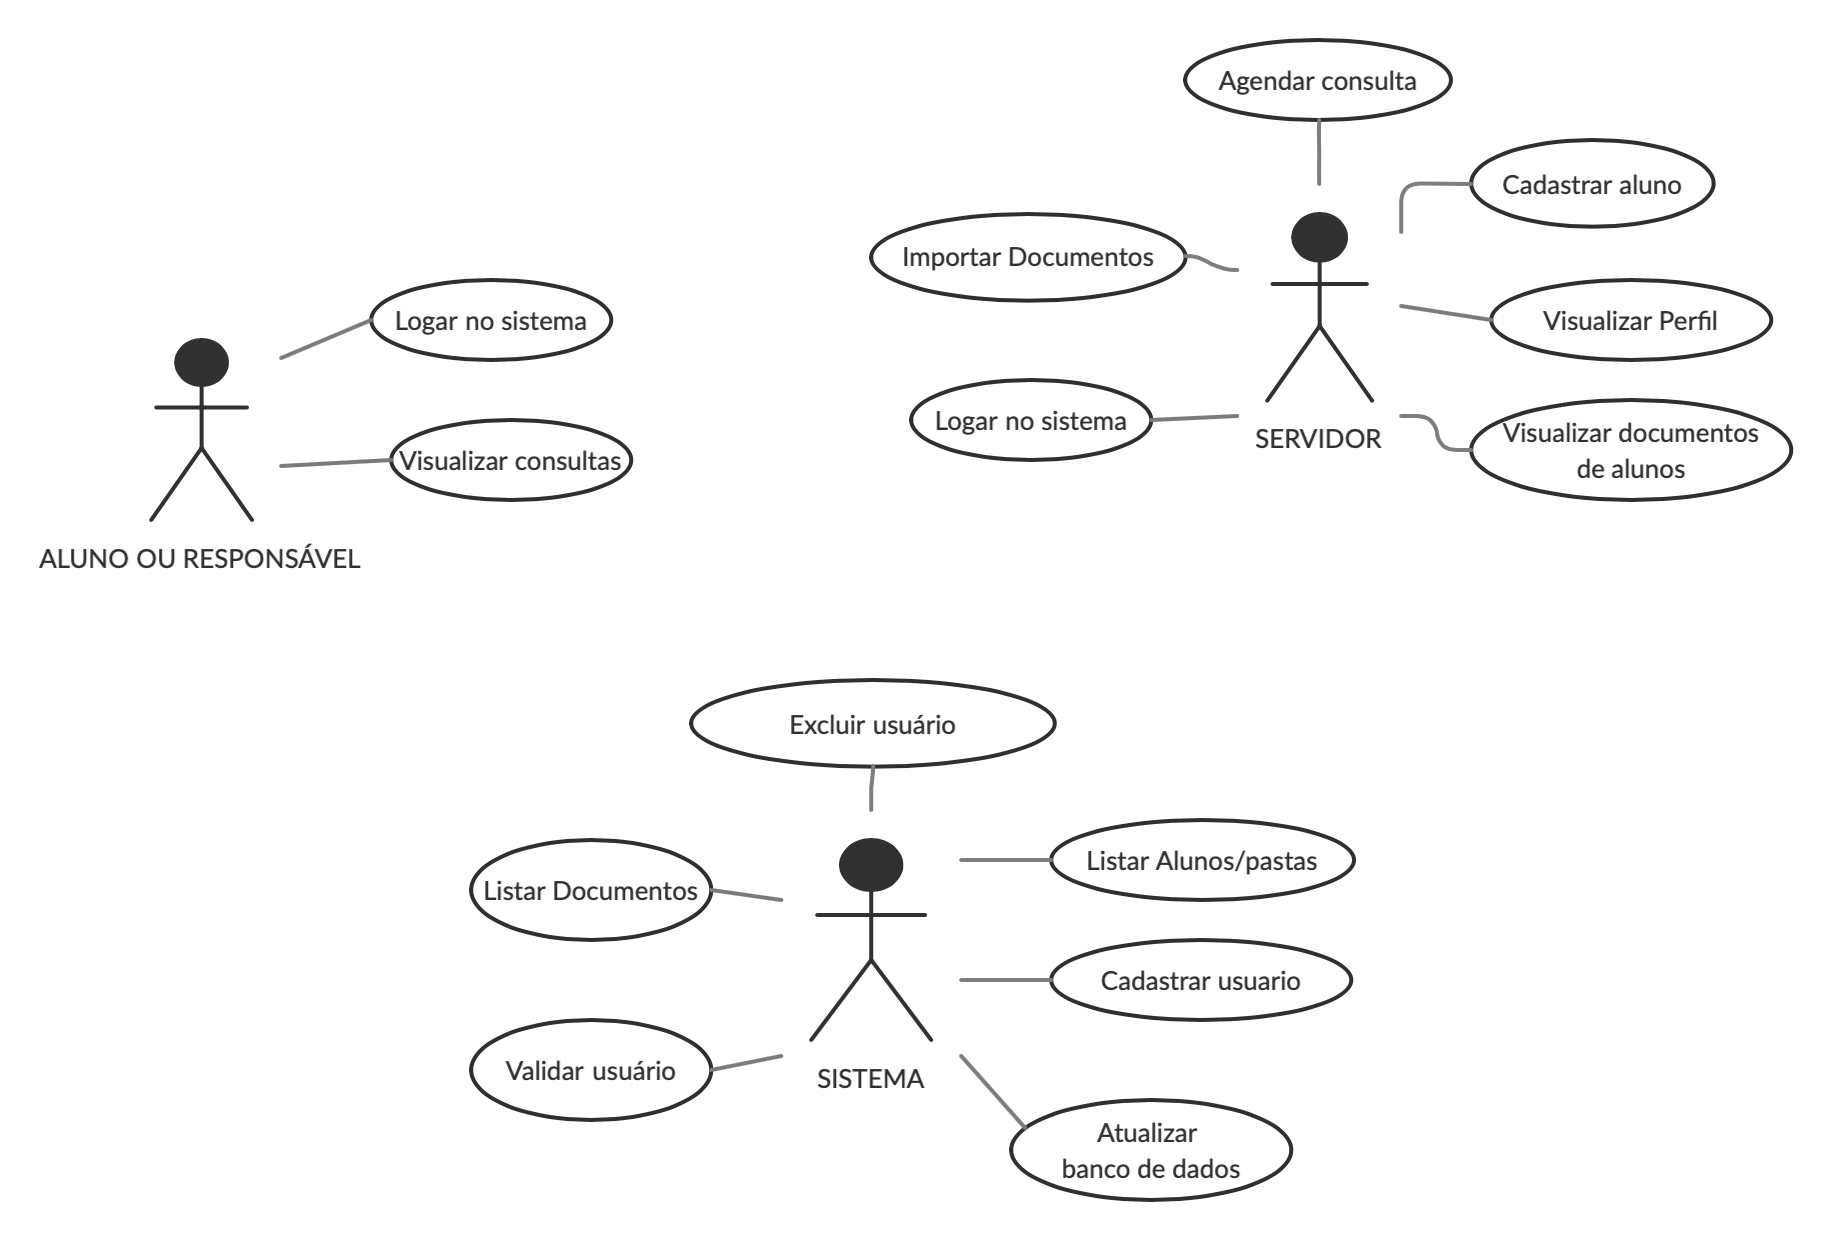
\includegraphics[width=1.0\textwidth]{./dados/figuras/Casos de uso}
    %\fonte{}
\end{figure}

\section{Levantamento de Requisitos}
\label{sec:requisitos}



%Metodologia---------------------------------------------------
\chapter{METODOLOGIA}
\label{chap:metodologia}

A fim de alcançar os objetivos propostos, a parte inicial desta pesquisa consiste em uma análise bibliográfica sobre a acessibilidade, buscando explorar experiências, regras e conhecimentos já existentes sobre o tema. 

O levantamento deste material teórico é de grande influência para a produção da ferramenta em questão tendo em vista que o projeto busca auxiliar o ambiente educacional aplicando os padrões de conteúdo acessível em um sistema para estudantes com NEE. 

Também é necessária a investigação sobre o ambiente educacional abordado pelo sistema, com informações qualitativas dos estudantes e dificuldades enfrentadas pelos profissionais do Campus. 

Para o desenvolvimento adequado do projeto, serão utilizados computadores com acesso à internet e tecnologias como:

\begin{enumerate}
    \item Kanban para gerenciamento ágil de tarefas;
    \item Linguagem de Programação Swift para o desenvolvimento da aplicação;
    \item Sketch para a etapa de prototipagem de telas;
    \item Framework XCTest para os testes unitários e de integração.
\end{enumerate}

Dentre as etapas do projeto, algumas já citadas acima, estão a etapa de Testes de UX/UI, onde os profissionais do Campus poderão opinar e expor ideias sobre a interface e o fluxo do sistema, o que guiará o design do projeto.                   % Metodologia
\include{estrutura/textuais/desenvolvimento/resultados}                    % Resultados
% ORIENTAÇÕES GERAIS------------------------------------------------------------

                   % Capítulo com Orientações de uso do Template
% CONCLUSÃO--------------------------------------------------------------------

\chapter{CONCLUSÃO}
\label{chap:conclusao}

Este capítulo tem o intuito de apresentar as contribuições do trabalho para a área de pesquisa e as possíveis metas a serem alcançadas.

\section{TRABALHOS FUTUROS}
\label{sec:trabalhosFuturos}

A intenção a longo prazo é ampliar o público-alvo deste projeto de forma que o mesmo sirva como modelo para instituições semelhantes de outros Campus, podendo auxiliar o trabalho de uma maior quantidade de profissionais e na assistência adequada aos estudantes. 

\section{CONSIDERAÇÕES FINAIS}
\label{sec:consideracoesFinais}
Tendo em vista o período dificultoso em que está sendo realizado este projeto de pesquisa, em meio à uma pandemia e isolamento social, é significativo que este projeto também tenha sua parcela de contribuição para uma assistência à distância em casos de situações posteriores e semelhantes a estas. 


\chapter{CRONOGRAMA}
\label{chap:cronograma}

Este capítulo apresenta o andamento e a estimativa de progresso durante o andamento do projeto, detalhando as etapas que serão efetuadas para atingir os objetivos desta pesquisa.

\begin{quadro}[!htb]
    \centering
    \caption{Cronograma de andamento do projeto 2020.2 - 2021.1
    \label{qua:quadro-exemplo1}}
    \begin{tabular}{|p{3cm}|p{1cm}|p{1cm}|p{1cm}|p{1cm}|p{1cm}|p{1cm}|p{1cm}|p{1cm}|p{1cm}|}
        \hline
        \textbf{Etapas} & \textbf{Jun} & \textbf{Jul} & \textbf{Ago} & \textbf{Set} & \textbf{Out} & \textbf{Nov} & \textbf{Dez} & \textbf{Jan}  & \textbf{Fev}\\
        
        \hline
        Escolha do tema & X &&&&&&&&\\
        \hline
        Revisão Bibliográfica & X & X &&&&&&&\\
        \hline
        Levantamento de Requisitos &&& X &&&&&&\\
        \hline
        Modelagem do Sistema &&& X &&&&&&\\
        \hline
        Processo de prototipagem &&& X &&&&&&\\
        \hline
        Testes UX &&& X & X &&&&&\\
        \hline
        Desenvolvimento &&&& X & X & X & X & X &\\
        \hline
        Testes de Código e UI &&&&& X & X & X & X & X\\
        \hline
    \end{tabular} %\fonte{\citeonline{Barbosa2004}}
\end{quadro}                 			   % Conclusão

\postextual
% INSERE ELEMENTOS PÓS-TEXTUAIS
% REFERÊNCIAS------------------------------------------------------------------

% Carrega o arquivo "base-referencias.bib" e extrai automaticamente as referências citadas

\bibliography{./base-referencias}
\bibliographystyle{abntex2-alf} % Define o estilo ABNT para formatar a lista de referências
% OBSERVAÇÕES------------------------------------------------------------------
% Este arquivo não precisa ser alterado.

\nocite{wcag2019, hig2020, ibge2020, IBGEeduca, design1997, relatorio2020}           			   % Referências
% APÊNDICES--------------------------------------------------------------------

\begin{apendicesenv}
\partapendices

% Primeiro apêndice------------------------------------------------------------
\chapter{Nome do apêndice} % Edite para alterar o título deste apêndice
\label{chap:apendiceA}

Lembre-se que a diferença entre apêndice e anexo diz respeito à autoria do texto e/ou material ali colocado.

Caso o material ou texto suplementar ou complementar seja de sua autoria, então ele deverá ser colocado como um apêndice. Porém, caso a autoria seja de terceiros, então o material ou texto deverá ser colocado como anexo.

Caso seja conveniente, podem ser criados outros apêndices para o seu trabalho acadêmico. Basta recortar e colar este trecho neste mesmo documento. Lembre-se de alterar o "label"{} do apêndice.

Não é aconselhável colocar tudo que é complementar em um único apêndice. Organize os apêndices de modo que, em cada um deles, haja um único tipo de conteúdo. Isso facilita a leitura e compreensão para o leitor do trabalho.

\end{apendicesenv}
             			   % Apêndices
% ANEXO------------------------------------------------------------------------

\begin{anexosenv}
\partanexos

% Primeiro anexo---------------------------------------------------------------
\chapter{Nome do anexo}     % edite para alterar o título deste anexo
\label{chap:anexoA}

Lembre-se que a diferença entre apêndice e anexo diz respeito à autoria do texto e/ou material ali colocado.

Caso o material ou texto suplementar ou complementar seja de sua autoria, então ele deverá ser colocado como um apêndice. Porém, caso a autoria seja de terceiros, então o material ou texto deverá ser colocado como anexo.

Caso seja conveniente, podem ser criados outros anexos para o seu trabalho acadêmico. Basta recortar e colar este trecho neste mesmo documento. Lembre-se de alterar o "label"{} do anexo.

Organize seus anexos de modo a que, em cada um deles, haja um único tipo de conteúdo. Isso facilita a leitura e compreensão para o leitor do trabalho. É para ele que você escreve.

\end{anexosenv}
               			   % Anexos

\end{document}
